% !TEX root = ./thesis.tex
\section{Survey of map generalization}

\subsection{Introduction}
% importance of maps
Since ancient times, mankind has created maps of the world based on whatever spatial information was available. Now and then, maps have been created for a plethora of purposes. From classical tasks such as navigation and education, to modern tasks such as finding shops near you or showing your friends on social media where you went jogging this afternoon.

% generalization
Although much has changed, the fundamental challenges posed by map creation remain largely the same. One of the key challenges of map creation is generalization. A geographical map will represent something as big as a planet or a country, on something as small as a sheet of paper or a computer screen. Map creators should eliminate information that is not essential to a map and reduce the visual complexity of the map as much as possible. This should be achieved without compromising the accuracy of what is conveyed too much. Striking a balance between these conflicting goals is at the core of what cartographers call generalization.

% challenge today
Today, huge amounts of spatial data is available to map creators, dwarfing the amounts of data available to map creators just a few decades ago. Furthermore, the frequency at which new maps must be created is higher than ever before, largely driven by the explosive rise in social media and online news platforms. Manual cartography can not keep up with this pace, and this has motivated many attempts to automate the generalization process. Researchers have achieved some degree of success with automatic generalization, but mostly for specialized domains such as points of interest and road networks. The definitive and fully general solution to automated map generalization has not been found.

% remainder
The remainder of this chapter is a survey of automated map generalization, with an emphasis on recent contributions to the field.


\subsection{Remainder}



This is a survey of cartographic generalization methods, in particular automatic methods for spatial data generalization. Cartography is the art of conveying spatial information using maps. Generalization is a subproblem of cartography when creating maps at a given scale. The main problems are to identify data subsets for display, and choosing appropriate rendering methods that effectively convey information at the given scale.


The purpose of map generalization is to maintain clarity, with appropriate content, at a given scale, for at chosen map purpose and intended audience~\cite{shea1989cartographic}. Many attempts have been made at automating the generalization process, but this is a difficult problem~\cite{frank1994multiscaletree}. While partial success have been achieved by recent systems~\cite{sarma2012fusiontables}, fully automated generalization remains an elusive goal.

The task of map generalization can be divided into two broad categories; The first is \emph{semantic generalization}, which is the task of affiliating individual features with classes in a semantic hierarchy such as a domain-specific thesauri~\cite{jones2005webage}. We will not deal with semantic generalization in this survey, but this may be looked at in future work (e.g. spatial classification based on machine learning over existing style layer descriptors). The second is \emph{geometric generalization}, which is concerned with simplification of the shape and structure of the graphical symbols that represent individual features~\cite{jones2005webage}. In this survey we exclusively review geometric generalization. If semantic generalization is a prerequisite of a particular method, it is assumed to be given.

% The main types of geometric transformation are: reduction in the number of discrete features that are portrayed (geometric selection); reduction in the detail of individual line, area and surface features (typically reduction in sinuosity); amalgamation of neighbouring features, whether point, line or area-referenced; reduction in dimensionality, or collapse, from area-referenced features to line or point referenced features; exaggeration of the size of significant features that would otherwise be too small to perceive; typification, or caricature, of the form and distribution of features that have been reduced in number to retain the original character; and displacement of the location of features to ensure that adequate separation distances are maintained between neighbouring features.

The individual transformations of geometric generalization will often impact upon each other. This interdependence between operations introduces the need for high-level procedures and optimization techniques to control the application of the individual operators~cite{jones2005webage}.
	
Automated generalization had always to compete with manual cartographers, therefore the manual generalization process was studied intensively~\cite{rieger1993consensus}. These studies resulted early in different generalization operators~\cite{brassel1988generalization,shea1989cartographic,gruenreich1992atkis}. By now there is no clear classification of operators available and it is doubtful if a comprehensive classification will evolve in future. The determination of generalization operators is known to be highly subjective; Rieger and Coulson conducted a study together with 23 cartographers which revealed areas of agreement and disagreement in the concepts these cartographers held regarding generalization and its procedures~\cite{rieger1993consensus}. Frank and Timpf note the problem of capturing interpreted importance, which generally makes the cartographic generalization an AI complete task~\cite{frank1994multiscaletree}.

To add more structure to the problem of automatic generalization, several formal models for automated generalization have been proposed in the past. These include: 

\begin{itemize}
\item McMaster and Shea model~\cite{shea1989cartographic}
\item Brassel and Weibel model~\cite{brassel1988generalization}
\item Gruenreich model~\cite{gruenreich1992atkis}
\end{itemize}

McMaster and Shea were among the first to look at digital cartographic generalization in a holistic way~\cite{shea1989cartographic}. They analyzed why we generalize, when to generalize and how to generalize, with a focus on when and how. They identified six conditions that occur under scale reduction, which may be used to determine a need for generalization. The conditions are reviewed in Section~\cite{sec:conditions}.

The separation between model generalization and cartographic generalization used in the Gruenreich model makes it most suitable for the current web-based and on-demand dissemination approach for data and maps of National Mapping Agencies~\cite{foerster2008classification}. We review the Gruenreich model in Section~\ref{sec:gruenreich-model}. 

We review some of the operators mentioned in the literature in Section~\ref{sec:generalization-operators} and review cartographic constraints in Section~\ref{sec:cartographic-constraints}.

\section{Generalization}

In this section we review the conditions and constraints that cause a need for generalization to arise. We also review the generalization operators that are applied in these situations, and finally we review a formal model for generalization, the Gruenreich model, that looks at the generalization problem at a higher level of abstraction.

\subsection{Types of generalization}
There are three types of generalization that are mentioned in the literature. \emph{Model generalization}, which aims at a reduction of detail for digital representation~\cite{haunert2006mip}, and \emph{cartographic generalization}, which creates visually pleasant maps~\cite{haunert2006mip}, and \emph{semantic generalization}, which is the task of affiliating individual features with classes in a semantic hierarchy such as a domain-specific thesauri~\cite{jones2005webage}.

\subsection{Conditions}
\label{sec:conditions}

Conditions arise as an effect of scale reduction. Conditions are the precursor to cartographic constraints, as they are the base cause why we need to generalize. McMaster and Shea consider six conditions~\cite{shea1989cartographic}. We have listed three conditions that depend only on the data, not on symbolization, below:

\begin{description}
\item [Congestion] As scale is reduced, the density of features per unit square increases. 

\item [Coalescence] As scale is reduced, features begin to touch because the given resolution is too coarse to represent the separation

\item [Imperceptibility] As scale is reduced, features may falls below a minimal portrayal size for the map.
\end{description} 

\subsubsection{Objective detection of conditions}

The conditions noted, however, are highly subjective in nature and, at best, difficult to quantify. Consider, for example, the problem of congestion. Simply stated, this refers to a condition where the density of features is greater than the available space on the graphic. One might question how this determination is made. Is it something that is computed by an algorithm, or must the we rely upon operator intervention? Is it made in the absence or presence of the symbology? Is symbology's influence on perceived density�that is, the percent blackness covered by the symbology the real factor that requires evaluation? What is the unit area that is used in the density calculation? Is this unit area dynamic or fixed? As one can see, even a relatively straightforward term such as density is an enigma. Assessment of the other remaining conditions coalescence, conflict, complication, inconsistency, and imperceptibility can also be highly subjective~\cite{shea1989cartographic}.

McMaster and Shea argue that in order to eliminate the subjective bias when evaluating whether a condition is reached, one must view the map as a graphic entity in its most elemental form: points, lines, and areas, and to judge the conditions based upon an analysis of those entities. This is accomplished through the evaluation of \emph{measures} which act as indicators into the geometry of individual features, and assess the spatial relationships between combined features. An incomplete list of measures taken from McMaster and Shea are:

\begin{description}
\item [Density measures] Number of point, line or polygon features per unit area, or number and location of cluster nuclei of point, line, or polygon features
\item [Distribution measures] These measures access the overall distribution of map features. For example, point features may be examined to measure dispersion, randomness, and clustering. Linear features may be accessed by their complexity, e.g. average angular change per unit length.
\item [Length and Sinuosity Measures] bla
\end{description}

\subsection{Models}

\subsubsection{Gruenreich model}
\label{sec:gruenreich-model}

The Gruenreich model~\cite{gruenreich1992atkis} provides a comprehensive view on automated generalization, and importantly separates the data from the maps and proposes a multi-stage generalization approach; from \emph{reality} to a \emph{dataset} or to a \emph{map} (see Table~\ref{fig:gruenreich}). 

Gruenreich identifies two types of generalization, namely model generalization used to obtain a data model at a lower level of detail and cartographic generalization used to obtain a readable map at a certain scale taking \emph{cartographic constraints} (see Section \ref{sec:cartographic-constraints}) into account.

\begin{figure}[htbp]
\label{fig:gruenreich}
\begin{center}
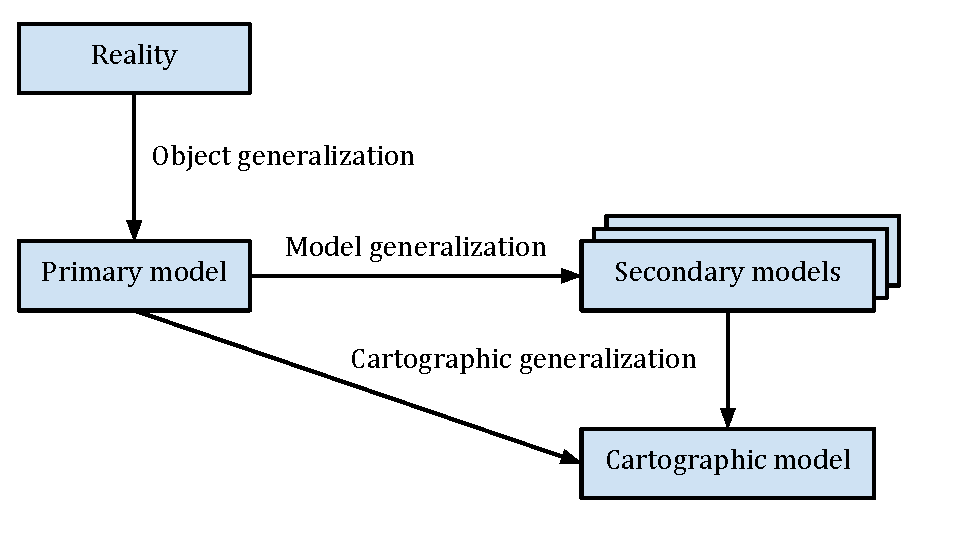
\includegraphics[scale=0.5]{figs/gruenreich.pdf}
\caption{Generalization model of Gruenreich. Reproduced from Foerster et al.}
\label{default}
\end{center}
\end{figure}

In the Gruenreich model there are two types of operators (see Section~\ref{sec:generalization-operators}); \emph{model generalization operators} and \emph{cartographic generalization operators}.

Other models do not provide such abstract view on generalization processing but describe more a fine-grain analysis of the logical and sequential~\cite{shea1989cartographic} or philosophic~\cite{brassel1988generalization} aspects of generalization processing.

It is important to note, that model generalization might be a pre-process for cartographic generalization, in which the user model for the visualization will be derived~\cite{foerster2007towards}.

\subsubsection{Other models}

Besides the established formal models for automatic generalization, different views on automated generalization have been established; the representation-oriented view~\cite{foo} and the process-oriented view~\cite{foo}. The first view focuses on the representation of data on different scales, which is related to the field of Multi-Representation Databases (MRDB)~\cite{foo,bar}. The latter view focuses on the process of generalization. 

\begin{figure}[htbp]
\begin{center}
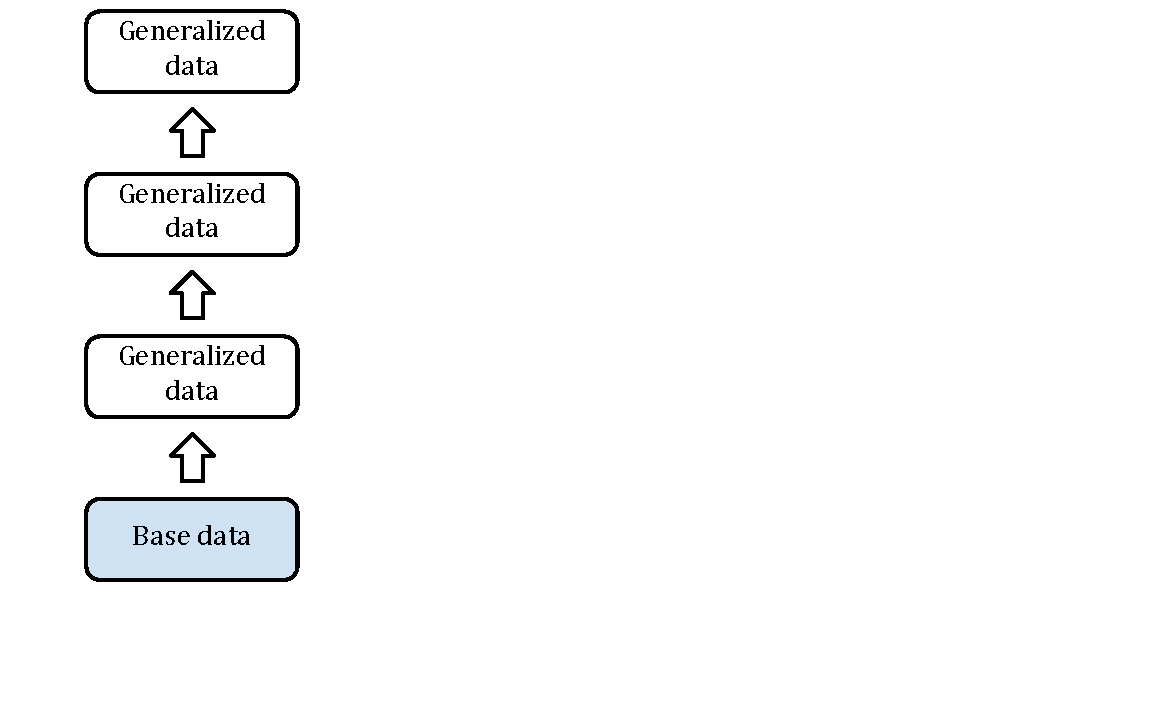
\includegraphics[scale=0.5]{figs/ladder.pdf}
\caption{Ladder-approach to generalization. Data is recursively derived from larger scales.}
\label{fig:ladder}
\end{center}
\end{figure}

The process of creating databases on different scales can be distinguished between the ladder and the star-approach. The ladder-approach is a stepwise generalization, in which each derived dataset is based on the other database of the next larger scale~\cite{foo}, see Figure~\ref{fig:ladder}. In the star-approach the derived data on all scales is based on a single (large-scale) data base~\cite{foo}, see Figure~\ref{fig:star}.

\begin{figure}[htbp]
\begin{center}
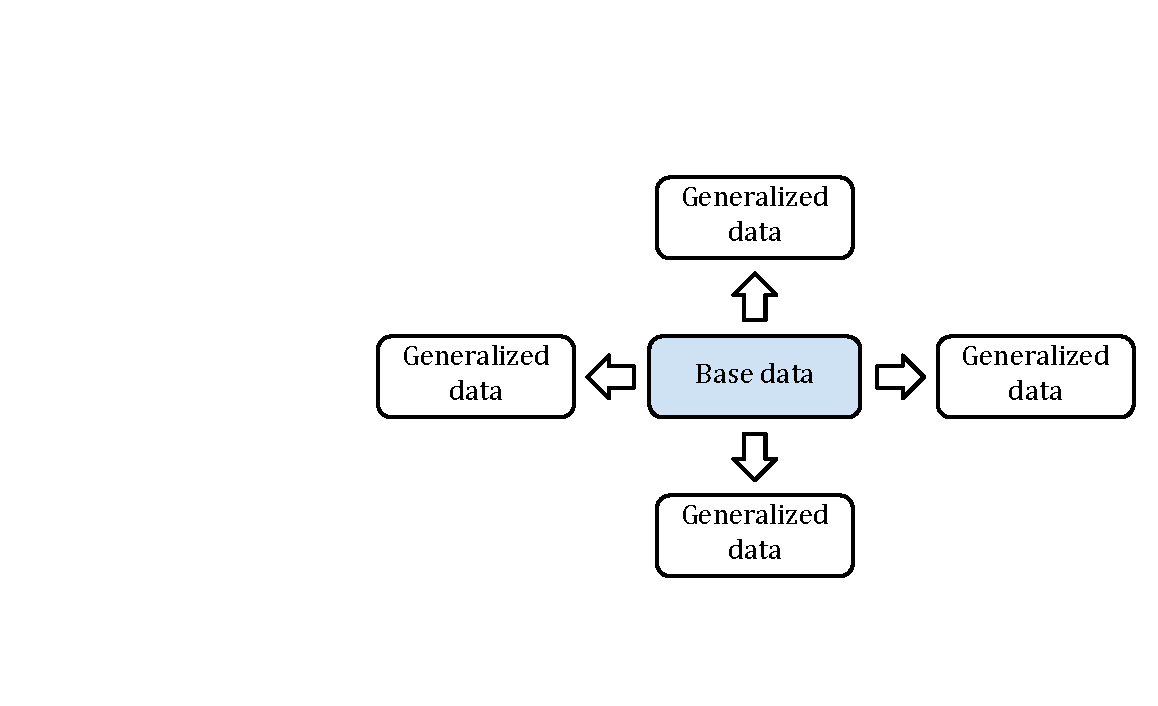
\includegraphics[scale=0.5]{figs/star.pdf}
\caption{Star-approach to generalization. Data at all scales is derived directly from base data.}
\label{fig:star}
\end{center}
\end{figure}


\subsection{Operators}
\label{sec:generalization-operators}
A generalization operator is an abstract description of a single action of the cartographer during manual generalization~\cite{foerster2008classification}. It is applied to single features, set of features or symbols representing features.

In the Gruenreich model there are two types of operators; model generalization operators and cartographic generalization operators. Model generalization operators are applied at the feature type level, while cartographic generalization operators are guided by globally defined constraints (see Section~\ref{sec:cartographic-constraints}), and are applied individually upon a group or single instances of features.

An operator is atomic in the sense, that it only affects well-defined and isolated aspects of a feature in an undividable way. Nevertheless, being atomic does not imply that such functionality is not without any side effects~\cite{foerster2008classification}.

The following is a non-complete list of operators copied from Wikipedia:

\begin{description}
\item [Selection] One way that geospatial data can be reduced is through the selection process. The cartographer can select and retain certain elements that he/she deems the most necessary or appropriate. In this method, the most important elements stand out while lesser elements are left out entirely~\cite{wikipedia2013generalization}

\item [Simplification] Generalization is not a process that only removes and selects data, but also a process that simplifies it as well. Simplification is a technique where shapes of retained features are altered to enhance visibility and reduce complexity~\cite{wikipedia2013generalization}

\item [Combination] Simplification also takes on other roles when considering the role of combination. Overall data reduction techniques can also mean that in addition to generalizing elements of particular features, features can also be combined when their separation is irrelevant to the map focus. A mountain chain may be isolated into several smaller ridges and peaks with intermittent forest in the natural environment, but shown as a contiguous chain on the map, as determined by scale~\cite{wikipedia2013generalization}

\item [Smoothing] Smoothing is also a process that the map maker can employ to reduce the angularity of line work. Smoothing is yet another way of simplifying the map features, but involves several other characteristics of generalization that lead into feature displacement and locational shifting. The purpose of smoothing is to exhibit linework in a much less complicated and a less visually jarring way. An example of smoothing would be for a jagged roadway, cut through a mountain, to be smoothed out so that the angular turns and transitions appear much more fluid and natural~\cite{wikipedia2013generalization}

\item [Enhancement] Enhancement is also a method that can be employed by the cartographer to illuminate specific elements that aid in map reading. As many of the aforementioned generalizing methods focus on the reduction and omission of detail, the enhancement method concentrates on the addition of detail. Enhancement can be used to show the true character of the feature being represented and is often used by the cartographer to highlight specific details about his or her specific knowledge, that would otherwise be left out. An example includes enhancing the detail about specific river rapids so that the map reader may know the facets of traversing the most difficult sections beforehand~\cite{wikipedia2013generalization}

\end{description}


\subsubsection{Operators in the literature}
Some authors classify their operators and other authors do not. McMaster and Yaolin et al. both lists six slightly different operators and do not classify them~\cite{mcmaster1989integration,yaolin2001frameworks}, see Table~\ref{tab:mcmaster-and-yaolin-operators}).

\begin{table}[htdp]
\caption{Operators by McMaster (1989) and Yaolin et al. (2001)}
\begin{center}
\begin{tabular}{|c|c|}
\hline
\textbf{McMaster (1989)} & \textbf{Yaolin et al.} \\
\hline
Simplification & Simplification (2001) \\
Merging & Merging \\
Enhancement & Aggregation\\
Displacement & Amalgamation \\
Smoothing & Classification \\
Omission & Selection \\
\hline
\end{tabular}
\end{center}
\label{tab:mcmaster-and-yaolin-operators}
\end{table}%

Other authors classify their operators with respect to a formal model like the Gruenreich model or the McMaster and Shea model. Foerster et al.~\cite{foerster2008classification} affiliate their ten operators with classifications in the Gruenreich model, see Table~\ref{tab:foerster-operators}.  

\begin{table}[htdp]
\caption{Operators by Foerster et al. (2007)}
\begin{center}
\begin{tabular}{|c|c|}
\hline
\multicolumn{2}{ |c| }{\textbf{Foerster et al.}} \\
\hline
\multirow{5}{*}{\emph{Model generalization}} & Class Selection \\
& Reclassification \\
& Collapse \\
& Combine \\
& Simplification \\
\hline
\multirow{4}{*}{\emph{Cartographic generalization}} & Enhancement \\
& Displacement \\
& Eliminiation \\
& Typification \\
\hline
\multirow{1}{*}{\emph{Both}} & Amalgamation \\
\hline
\end{tabular}
\end{center}
\label{tab:foerster-operators}
\end{table}%

Cecconi~\cite{cecconi2003integration} uses fifteen different operators with four operator classifications, see Table~\ref{tab:cecconi-operators}. McMaster and Shea use twelve operators and two classifications that are different from the Gruenreich classifications~\cite{shea1989cartographic}, see Table~\ref{tab:mcmaster-and-shea-operators}.

\begin{table}[htdp]
\caption{Operators by Cecconi (2003)}
\begin{center}
\begin{tabular}{|c|c|}
\hline
\multicolumn{2}{ |c| }{\textbf{Cecconi (2003)}} \\
\hline
\multirow{2}{*}{\emph{\textless Unspecified \textgreater}} & Thematic selection \\
& Thematic aggregation \\
\hline
\multirow{7}{*}{\emph{Individual objects}} & Weeding \\
& Unrestricted simplification \\
& Enlargement \\
& Exaggeration  \\
& Fractalization  \\
& Smoothing  \\
& Rectification  \\
\hline
\multirow{3}{*}{\emph{Individual or groups of objects}} & Selection \\
& Eliminiation  \\
& Displacement  \\
\hline
\multirow{3}{*}{\emph{Groups of objects}} & Amalgamation \\
& Combine  \\
& Typification  \\
\hline
\end{tabular}
\end{center}
\label{tab:cecconi-operators}
\end{table}%

\begin{table}[htdp]
\caption{Operators by McMaster and Shea (1989)}
\begin{center}
\begin{tabular}{|c|c|}
\hline
\multicolumn{2}{ |c| }{\textbf{McMaster and Shea}} \\
\hline
\multirow{10}{*}{\emph{Spatial transformations}} & Simplification \\
& Amalgamation \\
& Refinement \\
& Displacement \\
& Smoothing \\
& Merging \\
& Exaggeration \\
& Aggregation \\
& Collapse \\
& Enhancement \\
\hline
\multirow{2}{*}{\emph{Attribute transformations}} & Symbolization \\
& Classification \\
\hline
\end{tabular}
\end{center}
\label{tab:mcmaster-and-shea-operators}
\end{table}%

As should be evident, so many operators have been proposed, that it is unlikely that consensus will be achieved as to what the correct set of operators and operator classifications is. 

\subsubsection{Implementing operators}
Operators are implemented by different algorithms. For example, the simplification operator may be implemented by the Ramer-Douglas-Peucker algorithm~\cite{ramer1972iterative,douglas1973algorithms}, Visvalingam's algorithm~\cite{visvalingam1993line} or other algorithms. A comprehensive survey of operator algorithms is conducted in Section \ref{sec:implementing-operators}.

In an alternative view, an operator is implemented by a set of linear constraints and an objective function (see Section~\ref{sec:optimization-view}).

\subsection{Constraints}
\label{sec:cartographic-constraints}
Constraints have been formally introduced by Beard to replace complex rules for cartographic generalization; constraints define the state, which is assigned to single and groups of cartographic objects and should be maintained or reached in order to produce a readable map~\cite{buttenfield1991generalization}. In the Gruenreich model, cartographic constraints are used to guide the application of cartographic generalization operators.

Constraints are used in map-generalization control processes to produce the best result possible subject to the constraints. At a broad level, the objective of map generalization may be regarded as one of creating a map of a given scale that retains as much as possible of the relevant source information subject to cartographic considerations of \emph{legibility}. This objective can be quantified to some extent with respect to several factors that constitute constraints. These factors include topology, proximity, size, shape and pattern~\cite{jones2005webage}.

\subsubsection{T\"{o}pfer's Radical Law}
\label{sec:topfers-radical-law}
The visibility constraint is essentially T\"{o}pfer's Radical Law~\cite{topfer1966principles}, perhaps the most famous constraint. This is also known as the principle of constant information density. The Radical Law states that linear reduction in scale should amount to decrease in information according to geometrical progression. It is important to note that The Radical Law does not dictate exactly what information should be left out, only that some information should be left out. This constraint is also called the visibility constraint~\cite{sarma2012fusiontables}.

\subsubsection{Zoom consistency}
If a feature is visible at a lower scale, it must also be visible at all larger scales~\cite{sarma2012fusiontables}.

\subsubsection{Adjacency}
This constraint make most sense in a tile context. At a given scale, a given feature is either visible in all intersected tiles or none of them~\cite{sarma2012fusiontables}.

\subsubsection{Topology preservation}
Topological constraints are primarily concerned with the need to ensure that the simplified representations of the selected features retain original relationships of containment and connectivity~\cite{jones2005webage}.

\subsubsection{Size constraint}
Size constraints are intended to ensure that map symbols do not become too small to be clearly discernible~\cite{jones2005webage}.

\subsubsection{Proximity constraint}
Proximity constraints specify minimum separation distances between map symbols of various types and are intended to ensure that the individual symbols are easily distinguished from each other~\cite{jones2005webage}.

\subsubsection{Constraints of shape and pattern}
Constraints of shape and pattern are intended to preserve these original characteristics of individual features and of sets of neighbouring features. They are less easily formulated than the other constraints, as there are many ways in which these characteristics may be defined in terms of lower-level geometric parameters such as angularity, convexity, rectilinearity, elongation, collinearity, density and autocorrelation~\cite{jones2005webage}.

\subsubsection{Constraints from iOS6 Apple Maps}

These are constraints used when designing Apple Maps~\cite{nutanong2012multiresolution,samet2012duking}:

\begin{itemize}
\item Minimize overlaps
\item Respect relative importance of entries
\item Maximize spatial fullness (objective function?)
\item Provide panning/zooming consistency
\item Enable efficient sampling
\item Support filtering conditions
\end{itemize}

\subsection{Objective functions}

From Fusion Tables:

\begin{itemize}
\item Maximality
\item Fairness
\item Importance
\end{itemize}

\section{Implementing operators}
\label{sec:implementing-operators}

In this section we review how operators have been implemented in the literature. We begin by a brief review of specialized algorithms, like algorithms for simplification of line work, in Section~\ref{classic-algorithms}. In Section~\ref{optimization-approach}, we review approaches which target operator implementation more broadly, such as methods based on artificial intelligence or mixed integer programming~\cite{foo}.

Algorithms for operators are reviewed in the context of a pyramidal tile model~\cite{decola1993pyramid}. In this model, at a given scale, the plane is partitioned into uniform-sized cells or tiles, which form the unit of display on the map.

\subsection{Classic algorithms}
\label{sec:classic-algorithms}

\subsubsection{Simplification}
The algorithms by Ramer-Douglas-Peucker~\cite{ramer1972iterative,douglas1973algorithms} and Visvalingam~\cite{visvalingam1993line} simplify a single feature at a time, and do not take constraints such as topology preservation into account.

Examples of topology preserving algorithms are modifications of the Ramer-Douglas-Peucker~\cite{deberg1998topologically,saalfeld1999topologically} algorithm and algorithms based on constrained Delaunay triangulation~\cite{van2002characterisation,ai2000binary}.

The above mentioned algorithms generally work well for lines, but are not always appropriate for sets of polygons. Simplifying each boundary independently may result in glaring holes between adjacent polygons on a space-filling map. A better approach is to simplify all features in a single operation, by projecting line work onto a discrete grid. If adjacent points project onto the same grid location, they can be collapsed~\cite{lomet2012bigdata,giscloud,monnot2007optimization}.

\section{Optimization approaches}
\label{sec:optimization-approach}
The task of generalization of existing spatial data for cartographic production can be expressed as optimizing both the amount of information to be presented, and the legibility/usability of the final map, while conserving data accuracy, geographic characteristics, and aesthetical quality~\cite{monnot2007optimization}.

\emph{Our contribution, speculative}: Operators can often, if not always, be implemented as a set of linear constraints and an objective function.

TODO: \emph{Chapter 5: Control and optimization methods} of Map generalization in the Web age~\cite{jones2005webage} has a good review up to 2005.

\subsection{Real-time approach}

\subsubsection{Index traversal}

Adelfio et al.~\cite{nutanong2013efficient} and Nutanong et al.~\cite{nutanong2012multiresolution} (essentially the same paper). 


\subsection{Preprocessing approach}

\subsubsection{Simulated annealing}

ArcGIS~\cite{monnot2007optimization} and Ware et al.~\cite{ware2003sa}.

\subsubsection{Integer programming}

DeSarma et al. (Fusion tables)~\cite{sarma2012fusiontables} and Haunert et al. (landcover by mixed integer programming)~\cite{haunert2006mip}. 

These two in combination are very close to our case, i.e. good handling of points and of space-filling polygons (divided into classes and with aggregation).

\subsubsection{Neural networks}

Allouche et al.~\cite{allouche2005kohonen}

\subsubsection{Agent based modelling}
Lamy et al.~\cite{lamy1999application}.

